\documentclass{article}

% Cabecera del documento
% ======================================================================

% Paquetes extras
\usepackage[square, numbers, sort]{natbib}
% \usepackage{cite}
\usepackage{graphicx}
\usepackage[utf8]{inputenc}
\usepackage{amsmath,amssymb,amsfonts}
\usepackage{algorithmic}
\usepackage{textcomp}
\usepackage{subfig}
\usepackage{float}
\usepackage{mathtools}
\usepackage[spanish]{babel}
\usepackage[paper=a4paper,margin=2.75cm]{geometry}
\usepackage{booktabs} % for tables
\usepackage[colorlinks = true,
            linkcolor = blue,
            urlcolor  = blue,
            citecolor = orange,
            anchorcolor = blue]{hyperref} % for hyperlinks
\usepackage{xcolor} % text colors
\usepackage{minted}

% Directorio con imagenes
\graphicspath{{./figs/}}

% Cabecera del documento
% ======================================================================

% Titulo
\title{\textbf{CONTROL DE LA PRIMER ARTICULACIÓN DE ROBOT KR 10 R1100 sixx}}

% Autores
\author{Rodrigo Pérez \\ rodrigoperez2110@gmail.com \\ \\ Control y Sistemas, Facultad de Ingeniería, \\ Universidad Nacional de Cuyo, \\ Mendoza, Argentina}

% Fecha
\date{Junio de 2023}

% Cuerpo del documento
% ======================================================================
\begin{document}

% Comandos definidos por el autor
\renewcommand{\tablename}{Tabla}
% \renewcommand{\color{blue}{#1}}{\azul}

% Crear cabecera
\maketitle

% Resumen
% ======================================================================
% \begin{abstract}
%     El presente documento presenta los contenidos mínimos que debe tener el proyecto final de la cátedra de Control y Sistemas de la Universidad Nacional de Cuyo. Además, se aclara el estilo de redacción que debe tener el informe del proyecto final y se facilitan algunos recursos para la edición de documentos en \LaTeX.
% \end{abstract}

% Secciones
% ======================================================================
\section{OBJETIVO}
\label{sec:OBJETIVO}

% En la sección \ref{sec:intro}...

El presente proyecto tiene como objetivo diseñar y desarrollar el control de posición para el accionamiento electromecánico de la primer articulación del robot Kuka KR 10 R1100 sixx. El resultado esperado es lograr manipular correctamente la dinámica del robot, de forma tal que se obtenga a cada instante de tiempo la posición angular deseada de la primera articulación del mismo. Y lograrlo para cualquiera de los posibles valores de torque externo de carga mecánica del robot.


\begin{figure}[H]
    \centering
    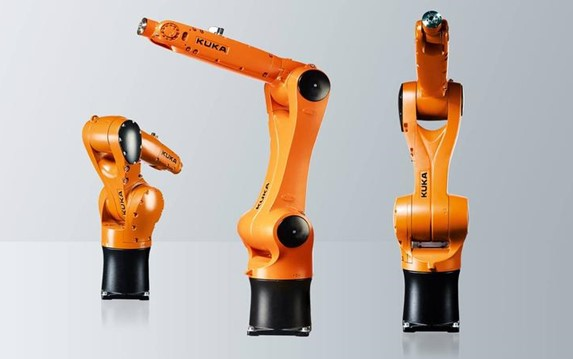
\includegraphics[width=1\textwidth]{3RobotsKuka}
    \caption{Robot Kuka KR 10 R1100 sixx}
    \label{fig:3RobotsKuka}
\end{figure}


% ======================================================================
\section{DESCRIPCIÓN}
\label{sec:DESCRIPCIÓN}


\subsection{MODELO DE LA PLANTA:}
\label{sec:MODELO DE LA PLANTA}

El robot Kuka elegido, es uno industrial tipo serie, de 7 eslabones, 6 articulaciones y 6 grados de libertad. Se selecionó dicho robot, ya que se trabajó particularmente con él en el proyecto final de la materia robótica 1, donde se obtuvieron las cinemáticas directa e inversa del mismo y se logró la simulación de su movimiento en MATLAB. Además, se ve a futuro de su uso en el proyecto final de carrera.

El proyecto se centrará en el control de la primer articulación del robot. El subsistema mecánico completo estará dado por el conjunto: articulación-reductor-motor. En donde para obtener el modelo matemático de la primera articulación, se debe tener en cuenta que, la posición, velocidad y aceleración de las demás articulaciones influyen en la dinámica de la primera. Esta influencia de las demás articulaciones da lugar a un modelo no lineal, pero en el presente proyecto se optará por aproximar dicho comportamiento no lineal de la carga mecánica, con un modelo linealizado que considera parámetros equivalentes variables. Dichos parámetros son:
\begin{itemize}
    \item Momento de inercia equivalente (variable):\\ Ya que, al cambiar el ángulo instantáneo de otra articulación, el momento de inercia, referido al eje de rotación vertical de la base inercial del robot, que experimentará la primer articulación variará.

    \item Amortiguamiento viscoso equivalente (variable):\\  Es una fricción ficticia, con la cual se logrará involucrar de forma equivalente los efectos de las fuerzas centrífugas y de Coriolis que aparecen cuando se mueven las demás articulaciones.
\end{itemize}

Al seguir dicha metodología, entonces se tendrá una incertidumbre en cuál es el valor de dichos parámetros, en función de cuál es el estado dinámico de las demás articulaciones. Lo que se representará en ambos parámetros equivalentes variables mediante un valor nominal ± una variación máxima.

Dicho modelado será verificado en simulación, y validado comparándolo con el robot real. Aunque a falta de disponer físicamente del robot, la validación del modelo matemático propuesto a controlar se realizará comparándolo con un modelo matemático más cercano a la realidad elaborado teniendo en cuenta las no linealidades del robot.

\begin{figure}[H]
    \centering
    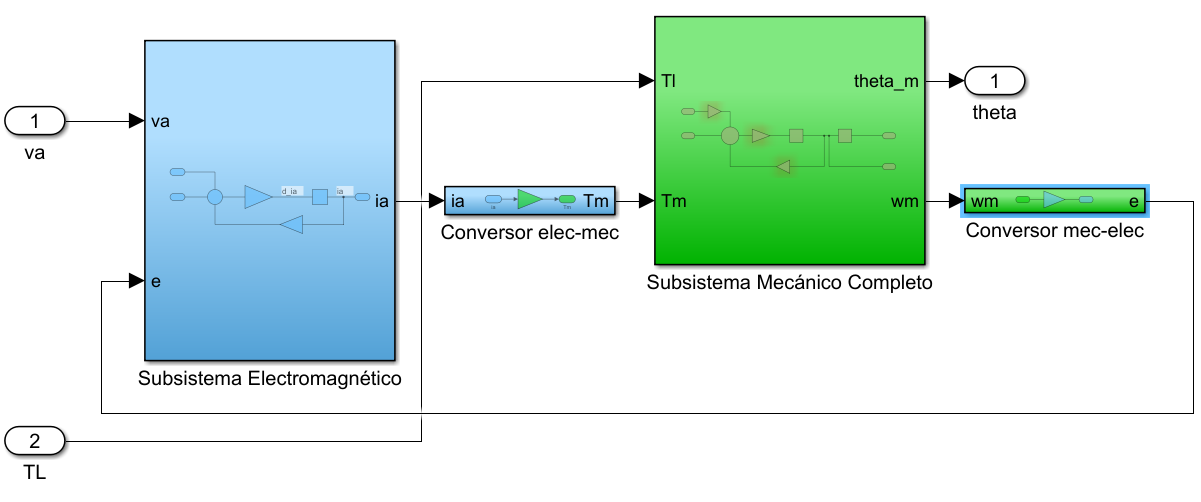
\includegraphics[width=1.1\textwidth]{Diagrama en bloques de la Planta}
    \caption{Diagrama en bloques de la Planta}
    \label{fig:Diagrama en bloques de la Planta}
\end{figure}


% ======================================================================
\subsection{CONTROLADOR:}
\label{sec:CONTROLADOR}

El sistema de control estará conformado por: una planta electromecánica, un controlador junto con la implementación de un observador de estados, un sensor de posición angular (encoder) y un filtro. Y el objetivo de dicho control será que el robot logre moverse sin oscilaciones, de una manera rápida y precisa, logrando brindar estabilidad y un correcto seguimiento de consignas.

El controlador que se propone es un controlador I-PD, con la idea de evitar desde un principio los problemas de amplificación de la señal de referencia que provocan la parte proporcional y derivativa, es decir, para evitar el Set-Point Kick. Esto se logra al colocar la ganancia proporcional y el bloque derivativo directamente en el lazo de realimentación, separados de la señal de referencia, como se muestra en la figura \ref{fig:Diagrama en bloques del Control (sin observador)}:

\begin{figure}[H]
    \centering
    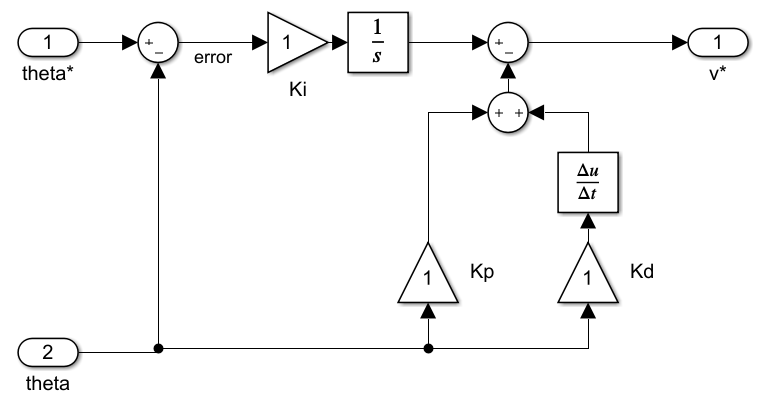
\includegraphics[width=0.60\textwidth]{Diagrama en bloques del Control (sin observador)}
    \caption{Diagrama en bloques del Control (sin observador)}
    \label{fig:Diagrama en bloques del Control (sin observador)}
\end{figure}

Como se puede ver en la figura \ref{fig:Diagrama en bloques del Control (sin observador)}, luego del bloque derivador se tiene la velocidad angular omega. Y como es conveniente no tener un bloque derivador (para evitar los problemas de amplificación de señal que conlleva la operación de derivación), se opta por eliminar este bloque derivador. Lo cual, es posible hacerlo al utilizar la variable omega estimada proveniente del observador. Es decir, que gracias a la implementación del observador, no se necesita derivar para obtener la velocidad angular. El diagrama de control quedará finalmente como se muestra en la figura \ref{fig:Diagrama en bloques del Control}.

\begin{figure}[H]
    \centering
    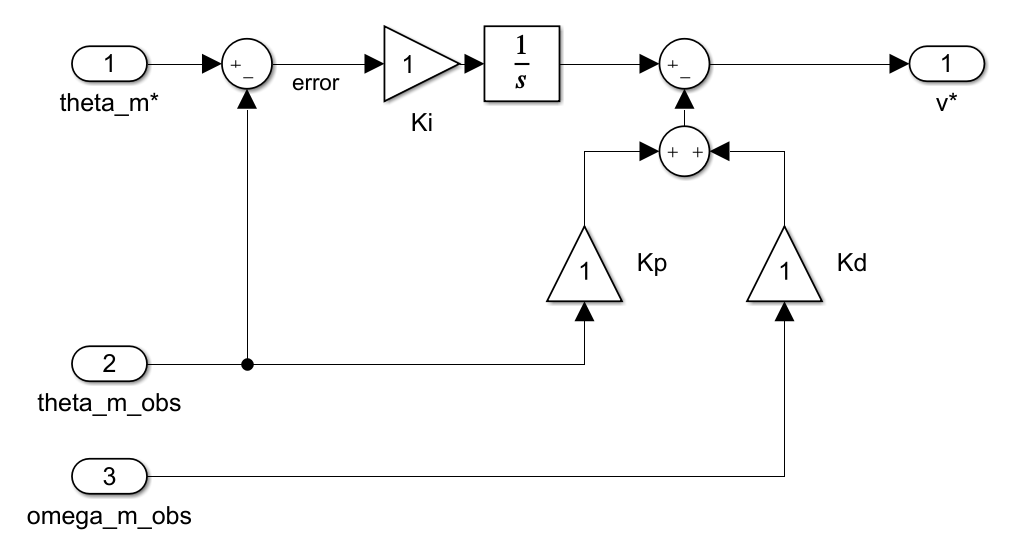
\includegraphics[width=0.60\textwidth]{Diagrama en bloques del Control}
    \caption{Diagrama en bloques del Control}
    \label{fig:Diagrama en bloques del Control}
\end{figure}

Además se modelará el sensor adicionando ruido blanco gaussiano, y se incorporará un filtro de tipo FIR en el lazo de realimentación para evitar la propagación de dicho ruido dentro del controlador.

Si resultara que el controlador I-PD porpuesto no lograra cumplir con los objetivos del proyecto, entonces se optará por un implementar alguna de las variaciones del controlador PID, como un controlador PID de dos grados de libertad.

El diagrama en bloques del sistema completo quedará como se muestra en la figura \ref{fig:Diagrama en bloques del Sistema Completo}:

\begin{figure}[H]
    \centering
    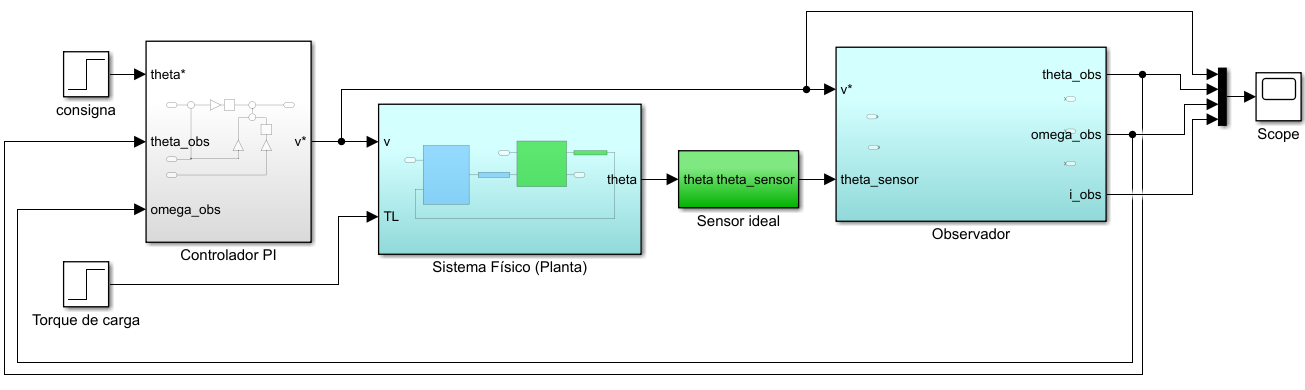
\includegraphics[width=1.1\textwidth]{Diagrama en bloques del Sistema Completo}
    \caption{Diagrama en bloques del Sistema Completo}
    \label{fig:Diagrama en bloques del Sistema Completo}
\end{figure}

El controlador se diseñará en tiempo continuo como se ha trabajado durante el cursado. Pero en la validación del modelo, el bloque del controlador será implementado en tiempo discreto con representación en punto fijo.
% ======================================================================


\section*{Bibliografía}

Wikibooks. Online \LaTeX{} book. \href{https://en.wikibooks.org/wiki/LaTeX/}{https://en.wikibooks.org/wiki/LaTeX/}.

Overleaf. Learn LaTeX in 30 minutes. \href{https://www.overleaf.com/learn/latex/Learn_LaTeX_in_30_minutes}{URL}.

Overleaf. Bibliography management in LaTeX. \href{https://www.overleaf.com/learn/latex/Bibliography_management_in_LaTeX}{URL}.

Franco Bizzotto. Proyecto: Modelado y diseño de controlador para robot serie redundante. \href{https://github.com/carloshernangarrido/control/blob/master/12_anteproyecto_proyecto-final/Bizzotto_Robot-serie.pdf}{URL}.


% Referencias
% ======================================================================

% Estilo de citas
\bibliographystyle{unsrt}




\end{document}
